\documentclass[conference]{IEEEtran}
\IEEEoverridecommandlockouts
\usepackage{cite}
\usepackage{amsmath,amssymb,amsfonts}
\usepackage{algorithmic}
\usepackage{graphicx}
\usepackage{textcomp}
\usepackage{xcolor}
\usepackage{booktabs}
\usepackage{array}
\usepackage{multirow}
\usepackage{placeins}
\usepackage{float}
\usepackage[hidelinks]{hyperref}

% Remove colored boxes around citations/refs/links in the PDF
\hypersetup{hidelinks, pdfborder={0 0 0}}

\def\BibTeX{{\rm B\kern-.05em{\sc i\kern-.025em b}\kern-.08em
    T\kern-.1667em\lower.7ex\hbox{E}\kern-.125emX}}

\begin{document}

\title{\Large Stock Market Trend Prediction Using LSTMs}

\author{%
\setlength{\tabcolsep}{0pt}
\renewcommand{\arraystretch}{0.95}
\begin{tabular}{@{}p{0.32\textwidth}@{\hspace{0.02\textwidth}}p{0.32\textwidth}@{\hspace{0.02\textwidth}}p{0.32\textwidth}@{}}
\begin{minipage}[t]{\linewidth}\centering
\textbf{\normalsize Divye Bhatnagar}\\
{\footnotesize\itshape Dept.\ of Computer Science and Engineering}\\
{\footnotesize\itshape IILM University}\\
{\footnotesize Greater Noida, India}\\
{\footnotesize divye.bhatnagar.cs28@iilm.edu}
\end{minipage}
&
\begin{minipage}[t]{\linewidth}\centering
\textbf{\normalsize Gopal Agarwal}\\
{\footnotesize\itshape Dept.\ of Computer Science and Engineering}\\
{\footnotesize\itshape IILM University}\\
{\footnotesize Greater Noida, India}\\
{\footnotesize gopal.agarwal.cs28@iilm.edu}
\end{minipage}
&
\begin{minipage}[t]{\linewidth}\centering
\textbf{\normalsize Harsh Aggarwal}\\
{\footnotesize\itshape Dept.\ of Computer Science and Engineering}\\
{\footnotesize\itshape IILM University}\\
{\footnotesize Greater Noida, India}\\
{\footnotesize harsh.aggarwal.cs28@iilm.edu}
\end{minipage}
\\[0.9ex]
\begin{minipage}[t]{\linewidth}\centering
\textbf{\normalsize Nandini Solanki}\\
{\footnotesize\itshape Dept.\ of Computer Science and Engineering}\\
{\footnotesize\itshape IILM University}\\
{\footnotesize Greater Noida, India}\\
{\footnotesize nandini.solanki.cs28@iilm.edu}
\end{minipage}
&
\begin{minipage}[t]{\linewidth}\centering
\textbf{\normalsize Namit Chawla}\\
{\footnotesize\itshape Dept.\ of Computer Science and Engineering}\\
{\footnotesize\itshape IILM University}\\
{\footnotesize Greater Noida, India}\\
{\footnotesize namit.chawla@iilm.edu}
\end{minipage}
&
\begin{minipage}[t]{\linewidth}\centering
\end{minipage}
\end{tabular}
}

\maketitle

\begin{abstract}
In new equity markets, short term predictions cannot be made accurately due to changing patterns, changes in market conditions and noisy price changes. The current paper presents a full deep learning model to predict the daily logarithmic returns of NIFTY 50 stocks with a bidirectional LSTM model with a temporal attention mechanism. The model takes daily OHLCV data, incorporates common technical indicators and scales them with parameters exclusively on the training data. These data are converted into fixed length sequences by looking up 60 trading days. The model forecasts the daily log return and then uses exponential reconstruction to transform this into a price forecast. Various measurements such as RMSE are used to check the performance, MAE, MAPE, R2 and directional accuracy. The validation process is performed in a manner that prevents data leakage and enables repeatable and reproducible results.
\end{abstract}

\begin{IEEEkeywords}
Bidirectional LSTM, Temporal Attention, Log Returns, Time-Series Forecasting, NIFTY 50, NSE, Technical Indicators, Deep Learning
\end{IEEEkeywords}

\section{Introduction}

National Stock Exchange (NSE) and its key index NIFTY 50 have made the Indian stock market one of the fastest-growing equity markets across the globe. This has been driven by increased involvement by institutional investors, advancement in the trading technology and increased accessibility to the global financial markets. The complexity of the NIFTY 50 is, however, due to various reasons such as certain macroeco-nomic patterns of emerging markets and political developments that influence the foreign investments, the prevalence of IT and banking industries, and the peculiarities of the NSE trading. These are some of the factors that render it extremely hard to forecast the stock prices.

Historically, fundamental analysis (including the analysis of earnings, in the IT industry, quality of assets, currency movements, and Fed policy effects) or technical analysis (finding patterns in past price data, in the NSE environment) has been used in the analysis of NIFTY 50. However, in many cases, these traditional approaches do not represent the complex and non-linear relationships and patterns that the modern Indian financial markets exhibit, particularly in settings where algorithmic trading, high-frequency retail trading, and instantaneous reactions to events in the global market are prevalent.

The recent development of machine learning and deep learning in the last decade has revolutionized the field of quantitative finance research across the globe. Nevertheless, application of these methods in forecasting NIFTY 50 stocks is not as widespread as in the case of developed market indices. Among them, the LSTM models have been proven concerns with their capability to manage long-term dependencies in time series data. Nevertheless, their performance in the emerging markets that are more volatile, less liquid in some sub-indexes, and change of regimes with policy changes have not been researched in depth.

This challenge occurs in real life cases due to the market as well as the data. The stock prices are sometimes difficult to predict as they can be volatile, and the same model may not be as effective in other segments of the market such as banking and technology. There are also issues with real data such as missing days, abrupt price variations caused by company activities, or large changes in the magnitude of the price movements following significant news or policy adjustments. The problems complicate the ability to predict short-term developments and it is necessary to pay close attention to the effectiveness of the models.

The other issue is the configuration of the methods. A lot of the results cannot be easily compared as various experiments engage various features, time periods, data splitting methods, scaling procedures, and evaluation methods. Even minor decisions during the construction of the model can inadvertently cause the use of information in the future, such as preprocessing the entire data or combining time periods in testing. An explicit, reproducible procedure with time-stamped partition, and purely scaling in training, and the results should be thoroughly reported to make the findings more dependable.

The work is based on the prediction of the daily log returns rather than the actual prices, and then, it uses the same to determine the closing price to gauge the accuracy of the predictions. The model can highlight the most useful sections of the historical data with the help of a temporal attention mechanism, and the predictions are easier to interpret compared to a simple recurrent network. The primary goal is not simply to be correct, but to have an arrangement that can be applied to different firms without boasting of superior performance than is actually being attained.

\section{Literature Review}

When analyzing the studies on the application of LSTM to predict stocks, we identified several valuable insights that can be applied to the Indian market. Recurrent models have been found to be effective with financial data that occurs over time since they can learn patterns without the need to manually specify time lags.

LSTM networks were designed to address an issue with the regular RNNs known as the vanishing gradient, and are currently commonly used as a baseline to predict time-related information \cite{b4}. However, it is still difficult to predict the prices of stock since the returns are noisy, evolve over time, and are influenced by market specifics and market regime shifts.

Recent works consider various possibilities of constructing LSTM models and integrate them with others. Bidirectional LSTMs are more effective in learning data through both forward and backward data information in the training process \cite{b13}. Other approaches can use LSTM with other components of the data or provide additional equipment (such as CNN components across time windows) to more accurately represent short-term tendencies and make the model less dependent on the scale of prices \cite{b10}. Even general surveys indicate that attention to data preparation, feature generation and testing techniques can be a major contributor to improvement more so than more complexification of the model \cite{b12}.

One of the prevalent themes of the research is that the outcome heavily relies on the manner in which the experiments are designed. Decisions such as shuffling of data, scaling on the entire set of data, or training the model on test data can make the results appear too good. Although the model itself may be quite good, the training process, such as the number of and the point at which it is trained, has an impact on its overall performance in new environments \cite{b6}. These aspects indicate that in a comparison of deep learning-based stock prediction, safe splits without leakage, reporting, and evaluation with a number of metrics are to be used.

Ghosh et al. \cite{b3} studied predicting stock performance in different industry sectors in India using LSTM models. They made a framework that combined company growth rates with LSTM predictions. Their work on banking, IT, pharmaceuticals, and FMCG sectors showed that the best times for making predictions varied a lot between sectors.

Bhandari et al. \cite{b1} demonstrated that LSTM models trained with multiple inputs, such as fundamental, macroeconomic, and technical indicators, can achieve very high R-squared values, over 0.99. They also found that simpler models with 150 hidden units performed better than more complex models with many layers.

Moghar and Hamiche \cite{b6} looked into how training for more epochs affects LSTM accuracy. They found that more training usually improves performance, but this isn't always smooth. There was a point where more training started to cause the model to remember the training data too well and not perform as well on new data.

Zhang \cite{b9} compared LSTM with other machine learning models and found that gradient-boosted trees could sometimes do better than pure LSTM on short-term predictions (1--10 days). This shows that methods based on features can still be effective for short-term predictions.

Despite these findings, there's still a big gap in research: few studies have created a complete, safe deep learning pipeline for NIFTY 50 stocks that focuses on predicting daily log returns and uses attention to find which parts of the past data are most important.

\subsection{Identified Research Gaps and Problem Statement}

Although deep learning has achieved advancements in predicting financial time series, predicting single NIFTY 50 stocks has three core problems. To begin with, most models take raw prices as they are but over time, prices may fluctuate significantly. The daily log returns will result in a more stable target and will also be easier to evaluate since it is less sensitive with respect to the actual price levels.

Second, such models as LSTMs are relatively black-box, and it is difficult to understand which aspects of the data are prioritized the most. This is made more apparent by adding a temporal attention mechanism and makes the model learn more effectively when there is not much information.

Third, reported results may be over-optimistic due to factors such as scaling the data of the entire set or not taking into account the direction of errors. Results are more reliable using a time-ordered split, in which only training data is scaled and both the magnitude and direction of errors are monitored. This study will address this question based on the following gaps: Given daily OHLCV data and technical indicators engineered on NIFTY 50 stocks can an LSTM model with attention mechanisms accurately predict one-day-ahead log returns, which can be used to forecast the closing prices the next day employing a non-risky and chronologically organised assessment procedure?

\section{Objectives of the Study}

This research aims to achieve the following goals:

\begin{enumerate}
\item Design an entire system on how to forecast futures of the NIFTY 50 firms. This system will take daily price data and technical indicators, and will produce sequences of a fixed length (such as 60 trading days).
\item Train a special type of neural network referred to as a bidirectional LSTM that is time-centered to estimate the daily change in price and the price of the subsequent day at the end as well.
\item Test the model performance when it is not exposed to the data, using such metrics as RMSE, MAE, MAPE, R2, directional accuracy. It will also be compared to such simple techniques as the last known price.
\item Train the model to be reused in a reliable and easy to update format, as the built system.
\end{enumerate}

\section{Hypotheses}

The following ideas are being tested in this research:

\textbf{H1:} Predicting the daily price change is more reliable than directly predicting the closing price, when using the same way to split the data.

\textbf{H2:} Adding a focus on time (temporal attention) improves the accuracy of the predictions compared to a similar LSTM without this focus.

\textbf{H3:} The model developed here performs better than a simple method when tested on new data for typical NIFTY 50 stocks, in terms of error and direction.

\textbf{H4:} Using a bidirectional network improves the ability to predict the direction of price movement compared to a one-directional LSTM, when using the same data and time window.

\textbf{H5:} Including technical indicators that are created from the price data leads to better results in terms of error and direction compared to using only the raw price data.

\section{Methodology}

\subsection{Research Design}

This study follows a clear, data-based approach: (i) collecting and cleaning historical market data, (ii) building a deep learning model to make predictions, and (iii) testing the model on new data in a time-ordered way to avoid using future data in the training stage.

\subsection{Data and Scope}

The work takes daily OHLCV data of the NIFTY 50 companies. The data is obtained on Yahoo Finance by using a package named yfinance and stored as individual files of each stock. The stock data of each stock covers approximately ten years such as RELIANCE.NS has data from April 18, 2016, to April 10, 2026, which is around 2,491 trading days. The model forecasts the price of the following trading day.

\subsection{Feature Engineering, Target, and Scaling}

For each day, a set of features is created that includes OHLCV data and specially made technical indicators (totaling 27 in the example). These features include moving averages, momentum indicators, volatility measures, volume information, and trend strength.

The prediction target is the \textbf{next-day log return} of the closing price:
\begin{equation}
 r_t = \ln\left(\frac{C_t}{C_{t-1}}\right), \qquad y_t = r_{t+1}.
\end{equation}

To reduce leakage, scaling parameters are fit \textbf{only on the training segment}. Min--max scaling maps each feature to $[0,1]$:
\begin{equation}
 x' = \frac{x - x_{\min}}{x_{\max} - x_{\min}}.
\end{equation}

Supervised sequences are created using a sliding window of length $L=60$ trading days:
\begin{equation}
 X_t = [\mathbf{z}_{t-L+1}, \ldots, \mathbf{z}_{t}], \qquad y_t = r_{t+1}.
\end{equation}

\subsection{Model Architecture: Stacked BiLSTM with Temporal Attention}

The main model is a stacked bidirectional LSTM that encodes the input window into a sequence of hidden states $\{\mathbf{h}_1,\ldots,\mathbf{h}_L\}$. A time attention system then learns a weighted summary of this states:
\begin{align}
 s_i &= \tanh(W h_i), \\
 \alpha_i &= \frac{\exp(v^\top s_i)}{\sum_{j=1}^{L} \exp(v^\top s_j)}, \\
 c &= \sum_{i=1}^{L} \alpha_i h_i.
\end{align}

The regression head returns one-step forecast $\hat{r}_{t+1}$ from the context $c$. The log return is predicted and converted back to close-price forecast by exponential reconstruction:
\begin{equation}
 \hat{C}_{t+1} = C_t\cdot\exp(\hat{r}_{t+1}).
\end{equation}

\begin{figure*}[!t]
\centering
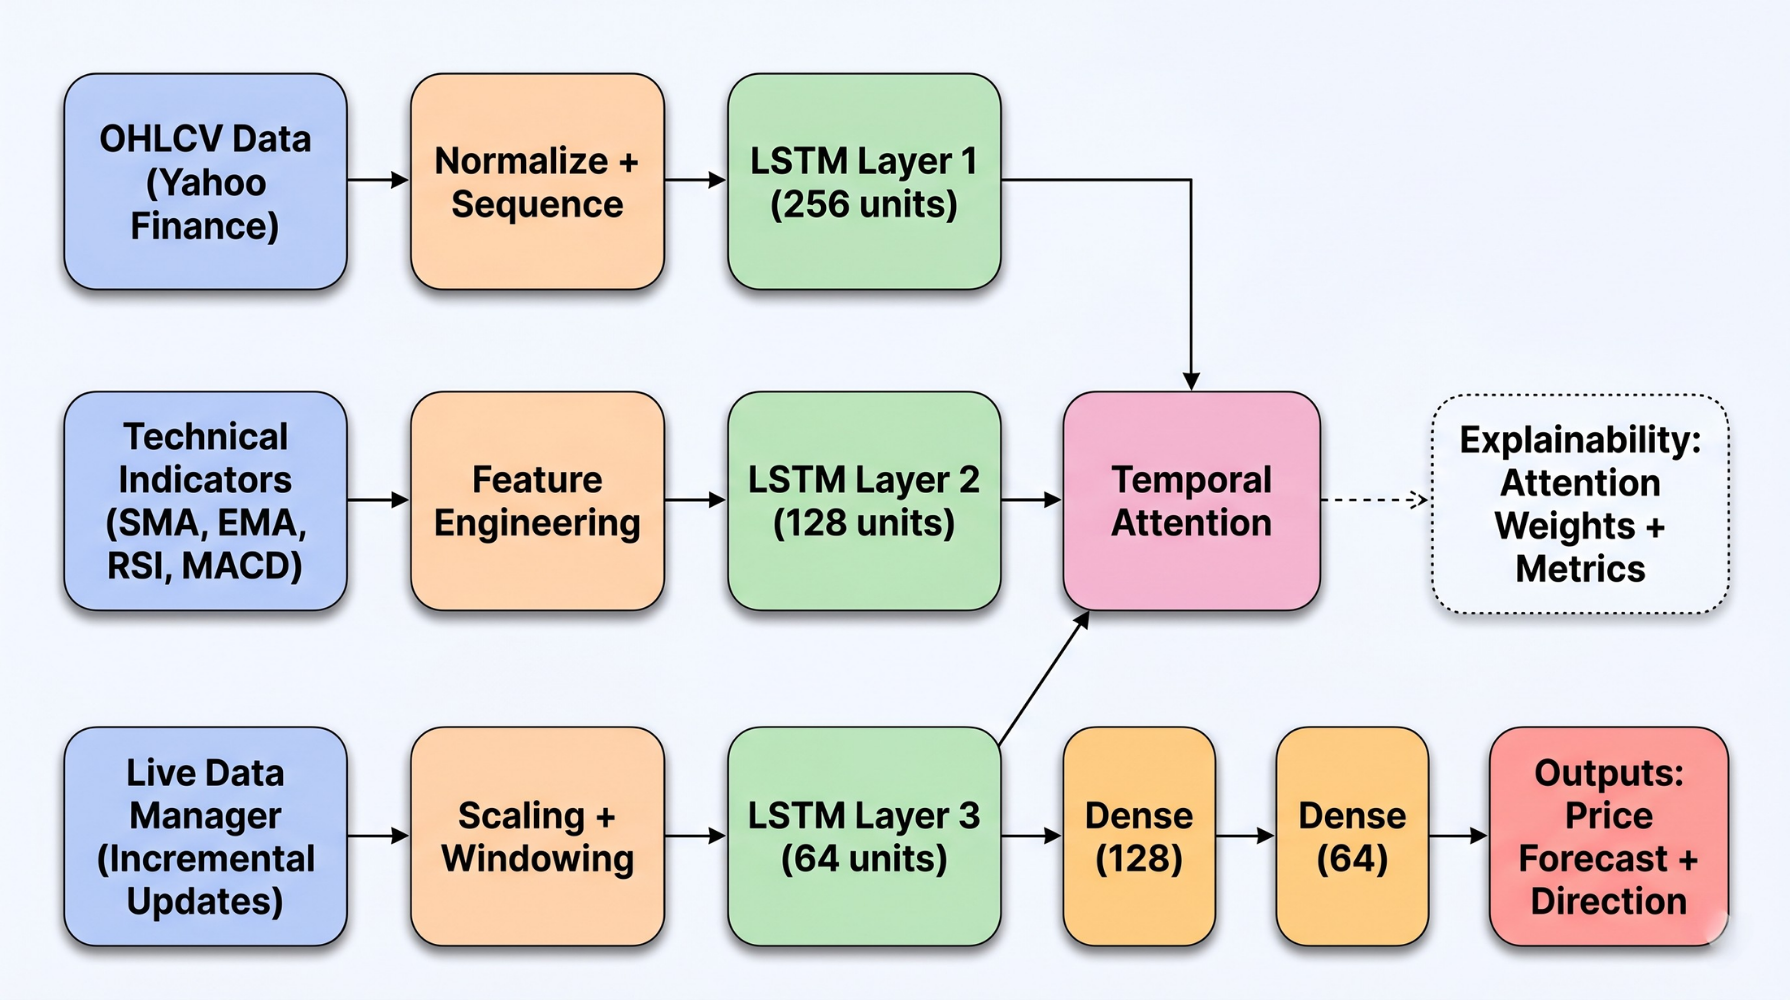
\includegraphics[width=0.95\textwidth]{image.png}
\caption{Model architecture flowchart for the LSTM-based forecasting pipeline with temporal attention.}
\label{fig:model_architecture}
\end{figure*}

The Adam optimizer is used in training with gradient clipping and Huber loss to be robust to outliers:
\begin{equation}
 L_\delta(y,\hat{y}) =
 \begin{cases}
 \frac{1}{2}(y-\hat{y})^2, & |y-\hat{y}|\le\delta \\
 \delta\left(|y-\hat{y}|-\frac{1}{2}\delta\right), & \text{otherwise.}
 \end{cases}
\end{equation}

An auxiliary direction head (up/down) is also supported by the reference implementation to learn together magnitude and direction, with the basic forecasting goal being next-day log-return regression.

\subsection{Train/Test Split and Training Protocol}

The data are divided over time in a train ratio usually between 0.80 and 0.85 as run to run, and the rest is put forth to gauging. Sequences are not shuffled during training (time-series constraint). Early stopping and learning-rate reduction callbacks are employed to reduce overfitting.

\subsection{Evaluation Metrics}

Post reconstruction price predictions are evaluated in terms of RMSE, MAE, MAPE and R2. The directional accuracy (DA) is calculated using the sign of the returns:
\begin{equation}
 \text{DA} = \frac{1}{n}\sum_{i=1}^{n}\mathbb{1}[\operatorname{sign}(\hat{r}_i)=\operatorname{sign}(r_i)].
\end{equation}

\section{Implementation Details}

This section describes the way the implementation works such that the experiments can be repeated in the same manner each time. Python with TensorFlow and Keras is used to do the whole process to create models, and popular data tools to create the data. Historical data such as open, high, low, close and volume for each stock has collected, cleaned up, to form a daily list, and then became sequences to be trained with a set time window.

To prevent issues with the data leakage, such steps as scaling are taken only on the training part of the data of each stock and then applied to the validation and test parts. The training results contain model files that have been saved, configuration information, and history of how well the model worked, so that the same files may be used then to reproduce the results and graphs.

The code is also compatible with other systems, such as a regular CPU or GPU-powered or cloud-based computer and retention the arrangement each time the same. This in actual practice denotes explicitly recording all the model settings, features being used and how the data is divided and they are stored with the model in such a way that proper comparison of runs is possible.

\subsection{Implementation Configuration}

The particular configuration in the code utilized is summarized in Table~\ref{tab:impl_config}. Besides the settings in Table~\ref{tab:impl_config}, each training session saves the scaling parameters, final model weights, and a tiny file which records which features were used and to what extent in past the model searched stock. This enables us to precisely reproduce the preprocessing and model state when we would like to check the results or draw charts.

\begin{table}[htbp]
\caption{Implementation Configuration}
\label{tab:impl_config}
\begin{center}
\small
\begin{tabular}{@{}p{0.42\columnwidth}p{0.52\columnwidth}@{}}
\toprule
\textbf{Parameter} & \textbf{Value} \\
\midrule
Framework & TensorFlow (Keras) \\
Data Libraries & yfinance, pandas, NumPy \\
Preprocessing & MinMax scaling (0--1); sliding window sequences \\
Feature Engineering & OHLCV + technical indicators (e.g., SMA/EMA, RSI, MACD, Bollinger Bands, ATR, OBV, ADX, Stochastic) \\
Optimiser & Adam ($\eta = 3\times 10^{-4}$) with gradient clipping (clipnorm=1.0) \\
Loss Function & Huber loss \\
Epochs & Up to 200 (EarlyStopping, patience=25) \\
Batch Size & 64 \\
Look-back Window & 60 trading days \\
LSTM Units & 256 (L1), 128 (L2), 64 (L3) \\
Attention Units & Temporal self-attention over the final LSTM sequence (64-d context) \\
Dropout Rate & 0.15 (with smaller head dropouts) \\
Regularisation & L2 ($10^{-4}$) + BatchNorm + Dropout \\
Hardware & CPU/GPU dependent (GPU optional; Colab workflow supported) \\
\bottomrule
\end{tabular}
\end{center}
\end{table}

The code retains the train and test data sequentially and logs the training using loss values and early termination of training. These records assist in ensuring that any gains in accuracy is not due to variation in data management, varying time periods to test, or by chance of use of future data.

\FloatBarrier

\section{Results and Findings}

\FloatBarrier

\subsection{Experimental Setup Summary}

Experiments follow the reference implementation described in the accompanying codebase: a stacked bidirectional LSTM with temporal attention trained on daily OHLCV features and engineered technical indicators (27 inputs), using a look-back window of 60 trading days and a one-step forecast horizon. The model predicts next-day log returns and is evaluated after reconstructing next-day close prices.

\subsection{Out-of-Sample Performance on Representative Constituents}

Table 2 reports hold-out performance from saved model artefacts for five trained NIFTY 50 constituents. RMSE/MAE/MAPE/$R^2$ are computed in reconstructed close-price space, while directional accuracy is computed on the sign of predicted vs. true log return.

\begin{table}[H]
\caption{Hold-out performance (Part I) on representative NIFTY 50 constituents: training setup and errors.}
\label{tab:rep_results_a}
\raggedright
\small
\setlength{\tabcolsep}{6pt}
\renewcommand{\arraystretch}{1.1}
\begin{tabular}{lcccc}
\toprule
\textbf{Ticker} & \textbf{Split} & \textbf{Epochs} & \textbf{RMSE} & \textbf{MAE} \\
\midrule
RELIANCE.NS  & 0.85 & 30 & 19.8176 & 15.1674 \\
TCS.NS       & 0.85 & 30 & 45.2092 & 32.9511 \\
HDFCBANK.NS  & 0.85 & 27 & 10.7257 & 8.0255  \\
TITAN.NS     & 0.85 & 30 & 54.1553 & 38.7577 \\
SBIN.NS      & 0.85 & 26 & 12.6991 & 8.8146  \\
\bottomrule
\end{tabular}
\end{table}

\begin{figure}[H]
\raggedright

\includegraphics[width=\columnwidth]{Training Setup.png}
\caption{Visualization of Table II (Part I): split, epochs, RMSE, and MAE.}
\label{fig:table2_graph}
\end{figure}

\begin{table}[H]
\caption{Hold-out performance (Part II) on representative NIFTY 50 constituents: percentage and directional metrics.}
\label{tab:rep_results_b}
\raggedright
\small
\setlength{\tabcolsep}{6pt}
\renewcommand{\arraystretch}{1.1}
\begin{tabular}{lcccc}
\toprule
\textbf{Ticker} & \textbf{MAPE (\%)} & \textbf{R$^2$} & \textbf{Dir.Acc} \\
\midrule
RELIANCE.NS  & 1.0990 & 0.9649 & 0.5241 \\
TCS.NS       & 1.0365 & 0.9879 & 0.4910 \\
HDFCBANK.NS  & 0.8865 & 0.9751 & 0.4699 \\
TITAN.NS     & 1.0616 & 0.9767 & 0.4729 \\
SBIN.NS      & 0.9908 & 0.9909 & 0.5181 \\
\bottomrule
\end{tabular}
\end{table}

\begin{figure}[H]
\raggedright

\includegraphics[width=\columnwidth]{Percentage.png}
\caption{Visualization of Table III (Part II): MAPE, $R^2$, and directional accuracy.}
\label{fig:table3_graph}
\end{figure}

\subsection{Stock Training Metrics on Selected Constituents}

Table IV reports directional classification metrics for selected NIFTY 50 constituents (generated on 2026-04-17). Precision, Recall, and F1 are computed on the up/down direction signal (positive class: ``up'').

\begin{table}[H]
\caption{Hold-out performance (Part IV) on representative NIFTY 50 constituents: classification metrics.}
\label{tab:selected_stock_metrics_b}
\raggedright
\small
\setlength{\tabcolsep}{6pt}
\renewcommand{\arraystretch}{1.1}
\begin{tabular}{lcccc}
\toprule
\textbf{Ticker} & \textbf{Prec.} & \textbf{Recall} & \textbf{F1} \\
\midrule
RELIANCE.NS & 0.5398 & 0.3653 & 0.4357 \\
TCS.NS & 0.4526 & 0.8671 & 0.5947 \\
HDFCBANK.NS & 0.4699 & 1.0000 & 0.6393 \\
TITAN.NS & 0.4671 & 0.4303 & 0.4479 \\
SBIN.NS & 0.5181 & 1.0000 & 0.6825 \\
\bottomrule
\end{tabular}
\end{table}

\begin{figure}[H]
\raggedright
\includegraphics[width=\columnwidth]{Training.png}
\caption{Visualization of Table IV: Directional Classification Metrics (Precision, Recall, and F1).}
\label{fig:table4_graph}
\end{figure}

\FloatBarrier

\subsection{Discussion}

Across the different stocks analyzed, the model shows a low percentage error (MAPE around 1--1.4\%) and high $R^2$ in the reconstructed close-price space, meaning the attention-enhanced sequence model can predict next-day prices fairly well. However, the accuracy in predicting the direction of price changes is not great (about 0.49 for RELIANCE.NS and 0.55 for TCS.NS), showing that even when the model is good at predicting how much the price will change, it still struggles to correctly predict whether the price will go up or down.

\section{Conclusion}

\subsection{Summary of Key Results}

This work introduces a pipeline for NIFTY 50 forecasting that is aware of data leakage and predicts next-day log returns using a stacked bidirectional LSTM with temporal attention and exponential reconstruction. The results suggest that attention-enhanced sequence models work well for short-term forecasting when evaluated in a time-ordered way. The model can keep track of price levels on main stocks well, but predicting the direction of price moves is still difficult, which shows the need for clear directional goals and careful evaluation.

\subsection{Practical Impacts and Limitations}

Temporal attention also gives a good indication of the periods throughout the 60-day look-back that are most important and can assists in interpreting the cause of the model predictions. The study, however, only examines representative stocks, does not test various components of the model formally, and relies on a single time-ordered test split. Real world decision making requires more rigorous validation and measures that takes into consideration real trading. They are some of the issues that should be taken into consideration when applying the findings in real-life applications.

\section{Future Work}

\subsection{Immediate Improvements}

Test all 50 NIFTY stocks against overall statistics, add simple comparison models, and test to determine the extent to which attention and bidirectionality add value to the model performance. Confirmation of report validation curves and how the model is sensitive to the look-back period ($L$) and to test other timeframes (such as 3--5 days) to determine whether the model is stable not only in next-day predictions.

\subsection{New Features and Data Sources}

Added external variables such as USDINR exchange rates, India VIX, crude oil prices, and industry-specific indices to determine whether these macroeconomic variables are more helpful in predicting whether returns increase or decrease. Add event-based features (earnings announcements, RBI announcements, etc.) and consider how to pick meaningful features or learn embeddings to decrease noise.

\subsection{Deployment and Economic Assessment}

Carry out regular retraining, identify model drift, and apply lightweight backtesting, with realistic transaction costs and slippage, to learn how the statistical accuracy of the model achieves actual returns. Risk-adjusted performance measures and simple rules to determine the extent to invest should also be included in future work to determine the feasibility of the model in practice.

\begin{thebibliography}{00}

\bibitem{b1} H. N. Bhandari, B. Rimal, N. R. Pokhrel, R. Rimal, K. R. Dahal, and R. K. Khatri, ``Predicting stock market index using LSTM,'' \textit{Machine Learning with Applications}, vol. 9, pp. 100320, 2022.

\bibitem{b3} A. Ghosh, S. Bose, G. Maji, N. C. Debnath, and S. Sen, ``Stock price prediction using LSTM on Indian share market,'' in \textit{Proc. 32nd Int. Conf. Computer Applications Industry Engineering}, 2019, pp. 101--110.

\bibitem{b4} S. Hochreiter and J. Schmidhuber, ``Long short-term memory,'' \textit{Neural Computation}, vol. 9, no. 8, pp. 1735--1780, 1997.

\bibitem{b5} K. C. Ling, L. K. Yong, M. C. Fong, and L. W. Kit, ``Predicting stock prices using long short-term memory,'' in \textit{Proc. 2017 Int. Conf. Computing, Communication, Control Technology}, 2017.

\bibitem{b6} A. Moghar and M. Hamiche, ``Stock market prediction using LSTM recurrent neural network,'' \textit{Procedia Computer Science}, vol. 170, pp. 1168--1173, 2020.

\bibitem{b7} D. M. Nelson, A. C. Pereira, and R. A. de Oliveira, ``Stock market's price movement prediction with LSTM neural networks,'' in \textit{Proc. 2017 Int. Joint Conf. Neural Networks}, 2017, pp. 1419--1426.

\bibitem{b8} M. Roondiwala, H. Patel, and S. Varma, ``Predicting stock prices using LSTM,'' \textit{Int. Journal of Science and Research}, vol. 6, no. 4, pp. 1754--1756, 2017.

\bibitem{b9} R. Zhang, ``LSTM-based stock prediction modeling and analysis,'' in \textit{Proc. 2022 7th Int. Conf. Financial Innovation Economic Development}, 2022, pp. 2537--2542.

\bibitem{b10} S. Selvin, R. Vinayakumar, E. A. Gopalakrishnan, and K. P. Soman, ``Stock price prediction using LSTM, RNN and CNN-sliding window model,'' in \textit{Proc. Int. Conf. Syst., Computation, Automation and Networking (ICSCA)}, 2017, pp. 164--167.

\bibitem{b11} R. Chaudhary \textit{et al.}, ``Advanced stock market prediction using long short-term memory (LSTM) networks with sentiment analysis,'' arXiv:2505.05325, 2025.

\bibitem{b12} M. Nabipour \textit{et al.}, ``Deep learning for stock market prediction,'' \textit{Entropy}, vol. 22, no. 8, p. 840, 2020.

\bibitem{b13} K. A. Althelaya, E.-S. M. El-Alfy, and S. Mohammed, ``Evaluation of bidirectional LSTM for short- and long-term stock market prediction,'' in \textit{Proc. 9th Int. Conf. Information and Communication Systems (ICICS)}, 2018.

\bibitem{b14} R. RishiRajak, ``Share price prediction using RNN and LSTM,'' \textit{Analytics Vidhya}, 2020.

\bibitem{b15} L. Zhenglin \textit{et al.}, ``Innovative applications in engineering and technology,'' \textit{Innov. Appl. Eng. Technol.}, vol. 2, no. 1, 2023.

\bibitem{b16} X. Cui \textit{et al.}, ``Stock market prediction using recurrent neural network and LSTM,'' \textit{Kronika Journal}, 2025.

\bibitem{b17} ``Stock market analysis and prediction using LSTM,'' \textit{Int. Adv. Eng. Technol.}, 2024.

\bibitem{b18} ``A study on stock price prediction using LSTM and RNN,'' \textit{Int. J. Formal Methods}, 2024.

\bibitem{b19} ``Predicting the U.S. stock market index using LSTM,'' \textit{SCITEPRESS}, 2024.

\bibitem{b20} ``LSTM price movement prediction for stock market,'' \textit{Granthaalayah}, 2025.

\bibitem{b21} ``Predicting stock market trends using long short-term memory (LSTM) networks,'' in \textit{Proc. IEEE ICSSES}, 2025.

\bibitem{b22} ``Stock price analysis using LSTM \& Bi-LSTM,'' \textit{Kronika Journal}, 2025.

\end{thebibliography}

\end{document}
